\chapter{Introduzione}

Negli ultimi anni, lo sviluppo di sistemi robotici autonomi sta avendo un ruolo sempre più importante in numerosi campi, ad esempio in ambito agricolo, 3D mapping, ampliamento della connesione Internet, consegna pacchi, industriale, ispezione e monitoraggio di luoghi \cite{UAVfuturo}. Una delle tecnologie più interessanti nel campo dei veicolo autonomi sono i veicoli aerei senza pilota (Unmanned Aerial Vehicles, UAV), comunemente chiamati droni. Essi risultano molto interessanti per la loro capacità di muoversi in ambienti complessi e di svolgere missioni in completa autonomia.
\\ \\
Uno dei requisiti affinché un drone possa svolgere missioni in autonomia è la capacità di saper determinale la propria posizione e posa nello spazio, poiche consentono ad esso di raggiungere degli obiettivi prestabiliti, mantenere una determinata posizione e di correggere la propria traiettoria durante il volo.
\\ \\
Una delle tecnologie più diffuse per la localizzazione degli UAV è il sistema globale di navigazione satellitare (Global Navigation Satellite System, GNSS), ad esempio il GPS. Tuttavia questo sistema presenta alcune limitazioni: la precisione, anche quando il GNSS è perfettamente disponibile, non è sufficiente se il drone deve navigare in spazi relativamente ristretti; inoltre la qualità del segnale può diminuire, risultare insufficiente o addirittura assente in presenza di ostacoli o in ambienti chiusi. \\
Queste limitazioni rendono necessario sviluppare delle alternative in grado di fornire posizione e posa del drone senza dipendere dai sistemi satellitari. Una possibile soluzione è quella di utilizzare strumenti per la navigazione basati sulla visione artificiale, ad esempio l'odometria visiva (Visual Odometry, VO); essi utilizzano una o più camere per analizzare l'ambiente, nell'obiettivo di stimare posizione e posa. In particolare, un possibile utilizzo della VO è quello basato sui marker, ovvero un marcatore fiduciale appositamente costruito per fornire varie informazioni come il suo ID, l'orientamento e la posizione nello spazio (esempio in Fig. \ref{fig:esempio_markers}). \\
Tutti i componenti necessari per il funzionamento del sistema (UAV, markers, companion computer,...) vengono rappresentati da un'unico sistema chiamato UAS (Unmanned Aircraft System).
\\
\begin{figure}
	\centering
	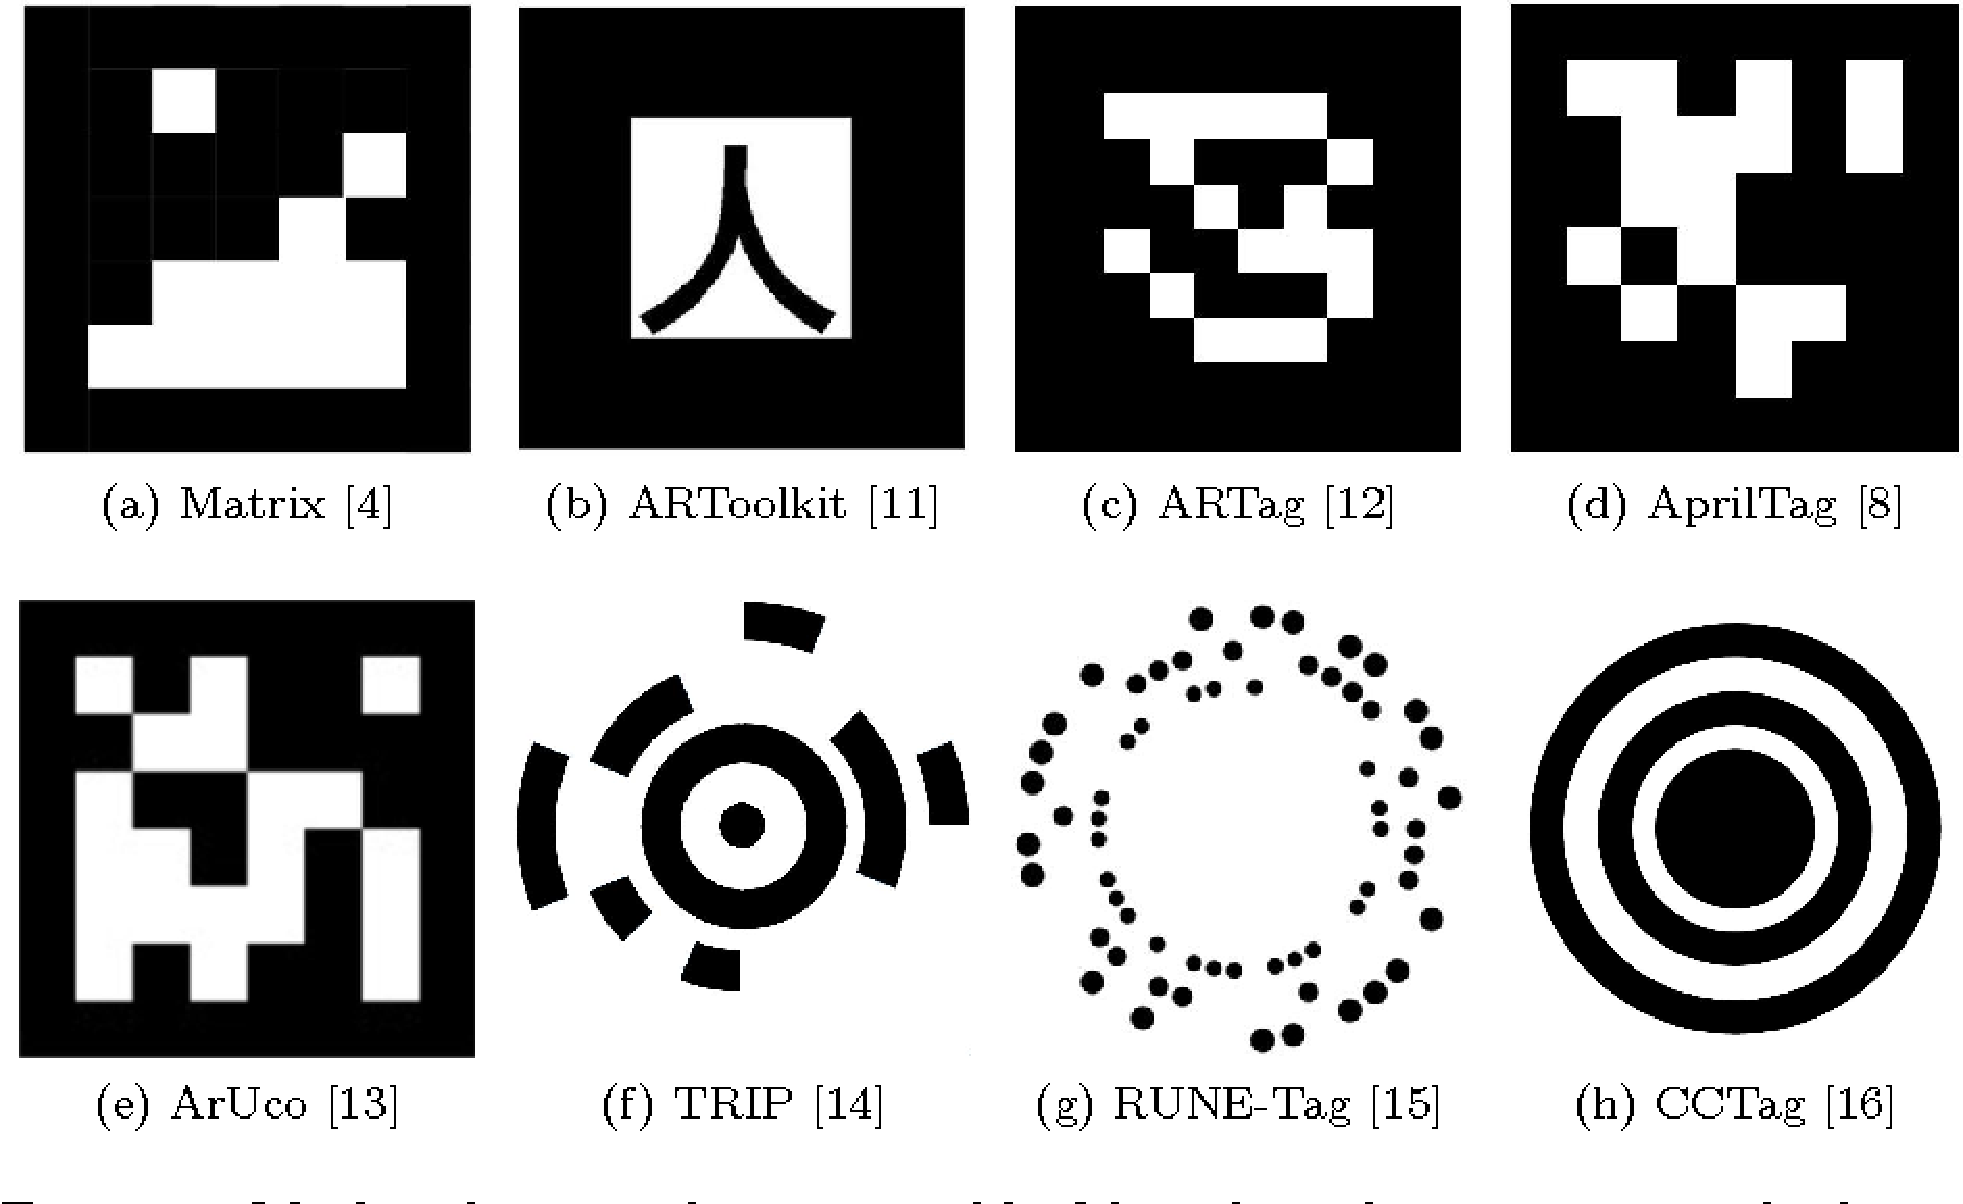
\includegraphics[width = 0.9\textwidth, trim={0 12mm 0 0}, clip]{immagini/esempio-markers.pdf}
	\caption{Esempio di marcatori fiduciali.}
	\label{fig:esempio_markers}
\end{figure}
\\
La tesi è strutturata nel seguente modo:
\begin{itemize}
	\item Capitolo \ref{chap:analisi_problema}: Analisi del problema\\
	Presenta un'analisi del problema da risolvere e la spiegazione ad alto livello della soluzione proposta.
	
	\item Capitolo \ref{chap:archi_sistema}: Architettura del sistema\\
	In questo capitolo viene affrontato in maniera dettagliata la struttura di tutto il sistema e delle varie scelte che sono state affrontate.
	
	\item Capitolo \ref{chap:prove_sperimentali}: Prove sperimentali\\
	Questa parte è dedicata ai test fatti sul simulatore e su un drone reale. Viene spiegato l'ambiente in cui i test vengono effettuati, la configurazione del drone e un'analisi dei risultati ottenuti.
	
	\item Capitolo \ref{chap:conclusione_sviluppi_futuri}: Conclusione e sviluppi futuri\\
	Infine nell'ultimo capitolo è presente una valutazione dei risultati ottenuti rispetto all'obiettivo prefissato; inoltre sono presenti delle proposte di miglioramento del sistema per eventuali sviluppi futuri.
\end{itemize}
